\sectionthree{Shift cipher}
\begin{python0}
from solutions import *; clear()
\end{python0}

This is one of the earliest cryptosystems and apparently Julius Caesar used it 
(high tech, eh?).
To encrypt a message, you simply do the following:
\[
\alpha \mapsto \delta, \ ...
\]
or in our alphabet system:
\begin{align*}
a &\mapsto d \\
b &\mapsto e \\
c &\mapsto f \\
\vdots &\textwhite{\mapsto d} \vdots 
\end{align*}
i.e. $a$ is replaced by $d$, $b$ is replaced by $e$, etc.
And of course you \lq\lq go around in a circle'': $x$ is replaced by $a$,
$y$ is replaced by $b$, $z$ is replaced by $c$.
\begin{align*}
a &\mapsto d \\
b &\mapsto e \\
c &\mapsto f \\
\vdots &\textwhite{\mapsto d} \vdots \\
x &\mapsto a \\
y &\mapsto b \\
z &\mapsto c
\end{align*}
This is known as the
\defone{Caesar cipher}.

Here's a simple Python code to encrypt a character:
\begin{console}[fontsize=\footnotesize]
def E(x):
    i = ord(x) - ord('a')
    i = (i + 3) % 26
    return chr(ord('a') + i)
\end{console}
and for \cpp:
\begin{console}[fontsize=\footnotesize]
char E(char x)
{
    return (x - 'a' + 3) % 26 + 'a';
}
\end{console}

Of course there's no reason why you must \lq\lq shift by 3''.
You can also shift by 7.
Right?
Note that the encryption input is only a single character.
Of course for a string, you just encrypt character-by-character.
Also, uppercase is replaced by lowercase.
Furthermore, 
anything not $a$-$z$ (example: punctuations, spaces) is thrown away.

Easy, right?
OK. Break the following the code:

\begin{center}
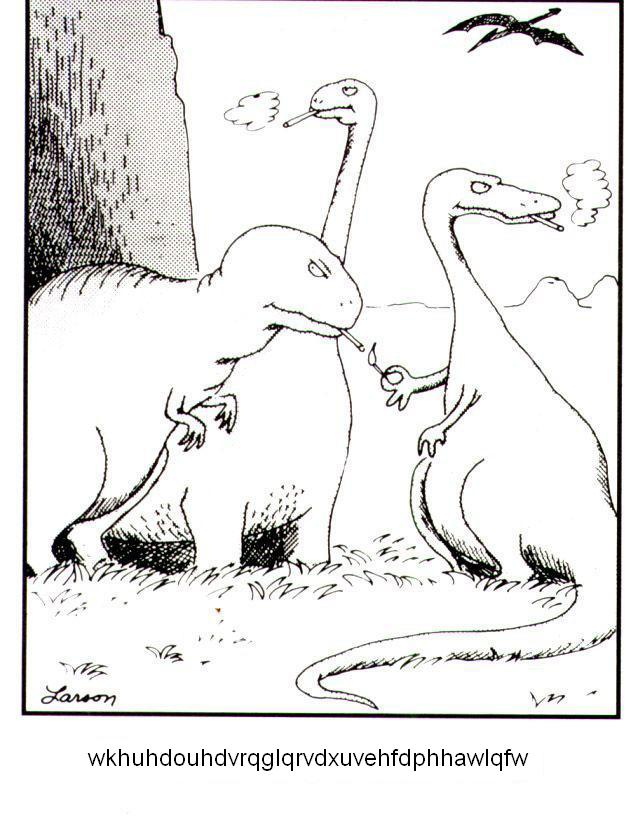
\includegraphics[width=5in]{dino-ciphertext.jpg}
\end{center}

\begin{center}
*** WARNING: SPOILERS ON THE NEXT PAGE *** 
\end{center}

\newpage
\begin{center}
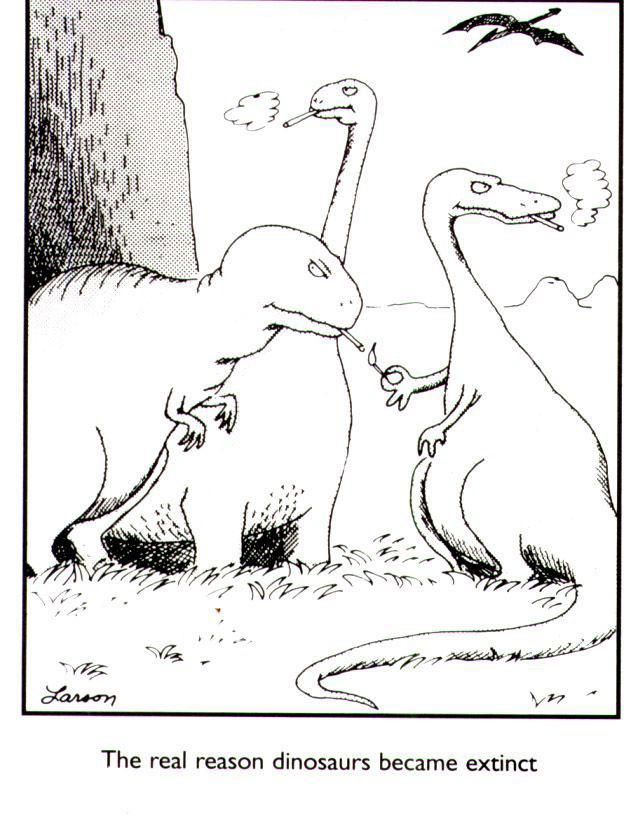
\includegraphics[width=5in]{dino-plaintext.jpg}
\end{center}


\begin{ex} 
  \label{ex:semigroup-associativity-0}
  \tinysidebar{\debug{exercises/{exercise-12/question.tex}}}
\mbox{}
  \begin{myenum}
  \item
    Solve
    \[
      5x^2 + y^2 = 3
    \]
    % mod 5, squares = 0^2=0, 1^2=1, 2^2=4, 3^2=4, 4^2=1
    (HINT: You don't really need number theory for this one. Why?
    But if you want to, imitate the solution for the previous
    problem.)
  \item
    Solve
    \[
      11y^2 - 5x^2 = 3
    \]
    % mod 5, squares = 0,1,4
    (HINT: This is just a slight change from the
    previous problem. \textit{But} now you need number theory. Try mod 4.
    If it does not work, try mod 5. Repeat.)
    % 3x^2 + y^2 = 3
    % {0,3} + {0,1} = 3
    % 0, 1, 3, 0 = 3
    % So x = 1, y = 0 (4)
    %
    % y^2=3 (5)
  \item
    Solve
    \[
      y^2 - 5x^2 = 2
    \]
    % mod 5, squares = 0^2=0, 1^2=1, 2^2=4, 3^2=4, 4^2=1    

  \item
    What about this one:
    \[
      x^2 - 5y^2 = 1
    \]    
  \end{myenum}
  {\scriptsize
[\textsc{Aside.}
Integer solutions to $x^2 - dy^2 = 1$ has been studied since at least 400BC.
This equation appear the Cattle Problem of Archimedes:

\begin{itemize}
  \item[]
If thou art diligent and wise, O stranger, compute the number of
cattle of the Sun, who once upon a time grazed on the fields of the
Thrinacian isle of Sicily, divided into four herds of different colours,
one milk white, another a glossy black, the third yellow and the last
dappled. In each herd were bulls, mighty in number according to these
proportions: Understand, stranger, that the white bulls were equal to
a half and a third of the black together with the whole of the yellow,
while the black were equal to the fourth part of the dappled and
a fifth, together with, once more, the whole of the yellow. Observe
further that the remaining bulls, the dappled, were equal to a sixth
part of the white and a seventh, together with all the yellow. These
were the proportions of the cows: The white were precisely equal to the
third part and a fourth of the whole herd of the black; while the black
were equal to the fourth part once more of the dappled and with it a
fifth part, when all, including the bulls went to pasture together. Now
the dappled in four parts8 were equal in number to a fifth part and a
sixth of the yellow herd. Finally the yellow were in number equal to
a sixth part and a seventh of the white herd. If thou canst accurately
tell, O stranger, the number of cattle of the Sun, giving separately the
number of well-fed bulls and again the number of females according
to each colour, thou wouldst not be called unskilled or ignorant of
numbers, but not yet shall thou be numbered among the wise. But
come, understand also all these conditions regarding the cows of the
Sun. When the white bulls mingled their number with the black, they
stood firm, equal in depth and breadth, and the plains of Thrinacia,
stretching far in all ways, were filled with their multitude. Again,
when the yellow and the dappled bulls were gathered into one herd
they stood in such a manner that their number, beginning from one,
grew slowly greater till it completed a triangular figure, there being
no bulls of other colours in their midst nor none of them lacking.
If thou art able, O stranger, to find out all these things and gather
them together in your mind, giving all the relations, thou shalt depart
crowned with glory and knowing that thou hast been adjudged perfect
in this species of wisdom.
\end{itemize}

If $W,X,Y,Z$ represents the number of white, black, yellow,
dappled bulls, you will get 
a systems of 7 linear equations, the first two being 
\begin{align*}
  W &= (1/2 + 1/3)X + Z \\
  X &= (1/4 + 1/5)Y + Z
\end{align*}
together with some constraints such as $W + X$ must be a square.
After some manipulations, it can be shown that the equation to solve looks like
\[
  x^2 - 410286423278424 y^2 = 1
\]
What was Archimedes thinking? You are find information on the Archimedes Cattle Problem on the web.]
}


  \solutionlink{sol:semigroup-associativity-0}
  \qed
\end{ex} 
\begin{python0}
from solutions import *
add(label="ex:semigroup-associativity-0",
    srcfilename='exercises/semigroup-associativity-0/answer.tex') 
\end{python0}


Let $P$ and $C$ be two sets.
A
\defone{cipher}
is just a pair of functions
$E: P \rightarrow C$ and $D: C \rightarrow P$
where $E$ is called the
\defone{encryption}
and $D$ is called the
\defone{decryption}
such that
\[
D(E(x)) = x \,\,\, \text{ for all } x \in P
\]
In other words
if you decrypt what you have encrypted, you get back the same data.
(It'd better be so!)
An element of $P$ is called a
\defone{plaintext} --
it's what you encrypt.
An element of $C$ is called a
\defone{ciphertext}
--
it's what you get when you encrypt.

Caesar cipher is an example of a cipher.
For Caesar cipher $P = C = \{a, b, c, ..., z\}$.
Also, although the encryption function maps one character to another,
it's understood that if you want to encrypt a string, you
simply encrypt each character of the string and join them up into
a string.

But if you allow the shift amount in the Caesar cipher to change,
then the encryption and decryption depends on the shift amount -- the key.
A general principle in cryptography is the following
concept due to
\href{https://en.wikipedia.org/wiki/Auguste_Kerckhoffs}{Auguste Kerckhoffs}:

\defone{Kerckhoffs' principle} (1883):
A secure cipher should not depend on the secrecy of the encryption
and decryption algorithm, but rather on the secrecy of the key.


The opposite and a really bad idea is called 
\defone{security through obscurity},
i.e., it's the hope that your
encrypted messages are safe as long as the encryption and decryption
algorithm are kept secret.

Why is this important?
Because it's easy to change the key while changing the encryption
and decryption algorithm might not be that easy.
If a worker who performs the encryption or decryption process is captured,
then he/she can be made (tortured?) to reveal the algorithm.
On the other hand, if the key is stolen, then we can simply change the key.
So in cryptography, it is always assumed that the algorithms (the cipher)
cannot be kept secret for long.

In fact in modern cryptography, once a cipher is designed,
the cryptography researcher(s) is expected to publish the cipher
so that other researchers can check if the cipher is actually secure.

So we just need to modify the definition of our cipher:

\begin{defn}
A
\defone{cipher}
is
a pair of functions
$E: K \times P \rightarrow C$ and
$D: K \times C \rightarrow P$ such that
if $k \in K$,
\[
D(k, E(k, x)) = x \,\,\, \text{ for all } x \in P
\]
$P$ is the set of plaintexts, $C$ is the set of ciphertexts,
and $K$ is the set of keys.
Notice that in the above the key used for encryption $k$
is the same as the key used for decryption.
\end{defn}

Instead of writing $E(k, x)$ and $D(k, x)$,
it's also common to write $E_{k}(x)$ and $D_{k}(x)$.
Depending on which book you read, the encryption and decryption functions
can also be written $e$ instead of $E$ and $d$ instead of $D$.

Humans have used ciphers for thousands of years.
The early ciphers always use the same key for encryption and decryption.
It was only very recently in 1970 that
\href{https://en.wikipedia.org/wiki/James_H._Ellis}{James H.~Ellis},
asked if it's possible to have a cipher that uses two distinct keys,
one for encryption and one for decryption.
Ellis was a British cryptographer at the
\href{https://en.wikipedia.org/wiki/GCHQ}{GCHQ }
(UK Government Communications
Headquarters).
If this is possible, then only the decyption key has to be kept secret.
Why do you want to a use such a cipher?

Well, I can publish the encryption key for such a cipher on a
website, you encrypt with the encryption key and send me the ciphertext by
email.
On receiving the ciphertext, I decrypt it using the decryption key.
Note that I can make the encryption key public, but I must keep
the decryption key a secret.
On the other hand for a symmetric key cipher, we would have to meet secretly
and decide on the common key.

Surprisingly such a cipher exists.

So now I have to modify our definition of ciphers ...

\begin{defn}
A
\defone{symmetric cipher}
is
a pair of functions
$E: K \times P \rightarrow C$ and
$D: K \times C \rightarrow P$ such that
if $k \in K$,
\[
D_k(E_k(x)) = x \,\,\, \text{ for all } x \in P
\]
$P$ is the set of plaintexts, $C$ is the set of ciphertexts,
and $K$ is the set of keys.
A symmetric cipher is also called a \defone{private key cipher}
because the key used must be kept private.
\end{defn}

And of course we also must have 

\begin{defn}
An
\defone{asymmetric cipher}
is a cipher where there are two distinct keys,
one for encryption and one for decryption.
An asymmetric cipher is also called a
\defone{public key cipher}
because the encryption key can be
made public (but the decryption key has to kept secret).
In this case, if $k,k'$ are the encryption and decryption keys,
then the cipher must satisfy
\[
D_{k'}(E_k(x)) = x
\]
for $x \in P$.
The encryption key $k$ is called the \defone{public key} (because it can be
made public)
while the decryption key is called the \defone{private key}.
\end{defn}


\begin{ex} 
  \label{ex:semigroup-associativity-0}
  \tinysidebar{\debug{exercises/{exercise-12/question.tex}}}
\mbox{}
  \begin{myenum}
  \item
    Solve
    \[
      5x^2 + y^2 = 3
    \]
    % mod 5, squares = 0^2=0, 1^2=1, 2^2=4, 3^2=4, 4^2=1
    (HINT: You don't really need number theory for this one. Why?
    But if you want to, imitate the solution for the previous
    problem.)
  \item
    Solve
    \[
      11y^2 - 5x^2 = 3
    \]
    % mod 5, squares = 0,1,4
    (HINT: This is just a slight change from the
    previous problem. \textit{But} now you need number theory. Try mod 4.
    If it does not work, try mod 5. Repeat.)
    % 3x^2 + y^2 = 3
    % {0,3} + {0,1} = 3
    % 0, 1, 3, 0 = 3
    % So x = 1, y = 0 (4)
    %
    % y^2=3 (5)
  \item
    Solve
    \[
      y^2 - 5x^2 = 2
    \]
    % mod 5, squares = 0^2=0, 1^2=1, 2^2=4, 3^2=4, 4^2=1    

  \item
    What about this one:
    \[
      x^2 - 5y^2 = 1
    \]    
  \end{myenum}
  {\scriptsize
[\textsc{Aside.}
Integer solutions to $x^2 - dy^2 = 1$ has been studied since at least 400BC.
This equation appear the Cattle Problem of Archimedes:

\begin{itemize}
  \item[]
If thou art diligent and wise, O stranger, compute the number of
cattle of the Sun, who once upon a time grazed on the fields of the
Thrinacian isle of Sicily, divided into four herds of different colours,
one milk white, another a glossy black, the third yellow and the last
dappled. In each herd were bulls, mighty in number according to these
proportions: Understand, stranger, that the white bulls were equal to
a half and a third of the black together with the whole of the yellow,
while the black were equal to the fourth part of the dappled and
a fifth, together with, once more, the whole of the yellow. Observe
further that the remaining bulls, the dappled, were equal to a sixth
part of the white and a seventh, together with all the yellow. These
were the proportions of the cows: The white were precisely equal to the
third part and a fourth of the whole herd of the black; while the black
were equal to the fourth part once more of the dappled and with it a
fifth part, when all, including the bulls went to pasture together. Now
the dappled in four parts8 were equal in number to a fifth part and a
sixth of the yellow herd. Finally the yellow were in number equal to
a sixth part and a seventh of the white herd. If thou canst accurately
tell, O stranger, the number of cattle of the Sun, giving separately the
number of well-fed bulls and again the number of females according
to each colour, thou wouldst not be called unskilled or ignorant of
numbers, but not yet shall thou be numbered among the wise. But
come, understand also all these conditions regarding the cows of the
Sun. When the white bulls mingled their number with the black, they
stood firm, equal in depth and breadth, and the plains of Thrinacia,
stretching far in all ways, were filled with their multitude. Again,
when the yellow and the dappled bulls were gathered into one herd
they stood in such a manner that their number, beginning from one,
grew slowly greater till it completed a triangular figure, there being
no bulls of other colours in their midst nor none of them lacking.
If thou art able, O stranger, to find out all these things and gather
them together in your mind, giving all the relations, thou shalt depart
crowned with glory and knowing that thou hast been adjudged perfect
in this species of wisdom.
\end{itemize}

If $W,X,Y,Z$ represents the number of white, black, yellow,
dappled bulls, you will get 
a systems of 7 linear equations, the first two being 
\begin{align*}
  W &= (1/2 + 1/3)X + Z \\
  X &= (1/4 + 1/5)Y + Z
\end{align*}
together with some constraints such as $W + X$ must be a square.
After some manipulations, it can be shown that the equation to solve looks like
\[
  x^2 - 410286423278424 y^2 = 1
\]
What was Archimedes thinking? You are find information on the Archimedes Cattle Problem on the web.]
}


  \solutionlink{sol:semigroup-associativity-0}
  \qed
\end{ex} 
\begin{python0}
from solutions import *
add(label="ex:semigroup-associativity-0",
    srcfilename='exercises/semigroup-associativity-0/answer.tex') 
\end{python0}


Public key ciphers use quite a bit of math.
So we won't see public key ciphers for a while.

Let's go back to our Caesar cipher.
You can think of the Caesar cipher as a special case of a symmetric cipher that
uses the key 3:
\begin{myenum}
\li encryption is \lq\lq shift forward by 3''
\li decryption is \lq\lq shift backward by 3''.
\end{myenum}
In other words, generalizing the Caesar cipher, we get the shift cipher:
\begin{myenum}
\li encryption is \lq\lq shift forward by $k$''
\li decryption is \lq\lq shift backward by $k$''.
\end{myenum}
where $k$ is the key.
I hope it's clear that the shift cipher with key 27 is
the same as the shift cipher with key 1.
Effectively speaking there are only 26 shifts, including
the very bad key of 0.
Hence for the shift cipher, $K = \{0, 1, 2, ..., 25\}$.

For classical ciphers, assuming we're only interested in English,
the plaintexts are
strings involving $a$-$z$.
I will write $\{a,b,c,...,z\}^*$ for the set of all strings with
characters from $\{a,b,c,...,z\}$.
If $n$ is a positive integer, I will also write $\{a,b,c,...,z\}^n$
for the set of strings with length $n$ and with characters
from the set $\{a,b,c,...,z\}$.
For instance
\[
\{a,b,c,...,z\}^2 = \{aa, ab, ac, ..., zx, zy, zz\}
\]


\begin{ex} 
  \label{ex:semigroup-associativity-0}
  \tinysidebar{\debug{exercises/{exercise-12/question.tex}}}
\mbox{}
  \begin{myenum}
  \item
    Solve
    \[
      5x^2 + y^2 = 3
    \]
    % mod 5, squares = 0^2=0, 1^2=1, 2^2=4, 3^2=4, 4^2=1
    (HINT: You don't really need number theory for this one. Why?
    But if you want to, imitate the solution for the previous
    problem.)
  \item
    Solve
    \[
      11y^2 - 5x^2 = 3
    \]
    % mod 5, squares = 0,1,4
    (HINT: This is just a slight change from the
    previous problem. \textit{But} now you need number theory. Try mod 4.
    If it does not work, try mod 5. Repeat.)
    % 3x^2 + y^2 = 3
    % {0,3} + {0,1} = 3
    % 0, 1, 3, 0 = 3
    % So x = 1, y = 0 (4)
    %
    % y^2=3 (5)
  \item
    Solve
    \[
      y^2 - 5x^2 = 2
    \]
    % mod 5, squares = 0^2=0, 1^2=1, 2^2=4, 3^2=4, 4^2=1    

  \item
    What about this one:
    \[
      x^2 - 5y^2 = 1
    \]    
  \end{myenum}
  {\scriptsize
[\textsc{Aside.}
Integer solutions to $x^2 - dy^2 = 1$ has been studied since at least 400BC.
This equation appear the Cattle Problem of Archimedes:

\begin{itemize}
  \item[]
If thou art diligent and wise, O stranger, compute the number of
cattle of the Sun, who once upon a time grazed on the fields of the
Thrinacian isle of Sicily, divided into four herds of different colours,
one milk white, another a glossy black, the third yellow and the last
dappled. In each herd were bulls, mighty in number according to these
proportions: Understand, stranger, that the white bulls were equal to
a half and a third of the black together with the whole of the yellow,
while the black were equal to the fourth part of the dappled and
a fifth, together with, once more, the whole of the yellow. Observe
further that the remaining bulls, the dappled, were equal to a sixth
part of the white and a seventh, together with all the yellow. These
were the proportions of the cows: The white were precisely equal to the
third part and a fourth of the whole herd of the black; while the black
were equal to the fourth part once more of the dappled and with it a
fifth part, when all, including the bulls went to pasture together. Now
the dappled in four parts8 were equal in number to a fifth part and a
sixth of the yellow herd. Finally the yellow were in number equal to
a sixth part and a seventh of the white herd. If thou canst accurately
tell, O stranger, the number of cattle of the Sun, giving separately the
number of well-fed bulls and again the number of females according
to each colour, thou wouldst not be called unskilled or ignorant of
numbers, but not yet shall thou be numbered among the wise. But
come, understand also all these conditions regarding the cows of the
Sun. When the white bulls mingled their number with the black, they
stood firm, equal in depth and breadth, and the plains of Thrinacia,
stretching far in all ways, were filled with their multitude. Again,
when the yellow and the dappled bulls were gathered into one herd
they stood in such a manner that their number, beginning from one,
grew slowly greater till it completed a triangular figure, there being
no bulls of other colours in their midst nor none of them lacking.
If thou art able, O stranger, to find out all these things and gather
them together in your mind, giving all the relations, thou shalt depart
crowned with glory and knowing that thou hast been adjudged perfect
in this species of wisdom.
\end{itemize}

If $W,X,Y,Z$ represents the number of white, black, yellow,
dappled bulls, you will get 
a systems of 7 linear equations, the first two being 
\begin{align*}
  W &= (1/2 + 1/3)X + Z \\
  X &= (1/4 + 1/5)Y + Z
\end{align*}
together with some constraints such as $W + X$ must be a square.
After some manipulations, it can be shown that the equation to solve looks like
\[
  x^2 - 410286423278424 y^2 = 1
\]
What was Archimedes thinking? You are find information on the Archimedes Cattle Problem on the web.]
}


  \solutionlink{sol:semigroup-associativity-0}
  \qed
\end{ex} 
\begin{python0}
from solutions import *
add(label="ex:semigroup-associativity-0",
    srcfilename='exercises/semigroup-associativity-0/answer.tex') 
\end{python0}


In modern day cryptography, we frequently work with bit strings.
The set of all bit strings is denoted by $\{0,1\}^*$.
Bit strings of length exactly 8 is denoted by $\{0,1\}^8$ --
these would be bytes.
For instance you might have heard of the SHA2 family of hash function.
SHA256 takes in bit strings and spits out bit strings of length 256.
So SHA256 is a function of type
\[
\{0,1\}^* \rightarrow \{0,1\}^8
\]
(Technically speaking SHA256 inputs do have a maximum limit in length,
but it's so huge that for practical purposes it's as good as all possible bit
strings.)

You know this is coming ... we'll be using
\textit{lots} of math to do 
encryption and decryption.
In particular, for this notes, we associate letters $a$ to $z$ with numbers.
The encryption and decryption function will work with either numbers of 
letters.
Specifically we have the following correspondence:
\sidebar{
In math, \lq\lq correspondence'' is the same as 
\lq\lq 1-1 correspondence'' which is the same as
\lq\lq bijection''.
Remember bijection?
It's time to check your discrete math notes}
\begin{align*}
a &\leftrightarrow 0 \\
b &\leftrightarrow 1 \\
c &\leftrightarrow 2 \\
\vdots  &\textwhite{\leftarrow 2} \vdots \\
z &\leftrightarrow 25
\end{align*}

if $E$ encrypts $a$ to $c$, I will say either 
\[
E(a) = c
\]
or 
\[
E(0) = 2
\]

Now you might say ... \lq\lq so what's the big deal? 
Why rewrite $a$ as $0$,  $b$ as $1$, etc.
I can also come up with some secret encoding for instance
why can't I rewrite $a$ as a square, $b$ as a triangle, etc.?''

Well ... the reason is because $0, 1, 2, ...$ are numbers ... and ...
\textit{they have operations (addition, subtraction, multiplication, division).}

With the above in mind, instead of describing the shift cipher as
functions on $a$-$z$, I'll describe it as function on $\Z/26$:

\begin{defn}
The \defone{shift cipher} $(E, D)$ is given by
\[
  E_k(x) = x + k \pmod{26}
\]
and
\[
  D_k(x) = x - k \pmod{26}
\]
\end{defn}

It's clear that for the shift cipher $(E, D)$,
\[
D_k(E_k(x)) \equiv x \pmod{26}
\]

And of course the shift cipher with key $k = 3$ is the \defone{Caesar cipher}.
